\title{Syntax and Semantics Exam}
\author{
        Benjamin Bennetzen \\
        Student ID: 20204861 \\
        Computer Science, 4th semester\\
}
\date{\today}

\documentclass[12pt]{article}

\usepackage{tikz}
\usepackage{listings}
\usepackage{mathpartir}
\usepackage{ebproof}
\usepackage{amsmath}
\usepackage[utf8]{inputenc}
\usepackage{amssymb}
\usepackage{graphicx}
\usepackage{stmaryrd}

\newcommand{\R}{\mathbb{R}}
\newcommand{\F}{\mathbb{F}}
\newcommand{\num}[1]{\mathcal{N}\llbracket #1 \rrbracket}

\begin{document}
\maketitle

\section{Exercise}
\subsection{}
\begin{center}
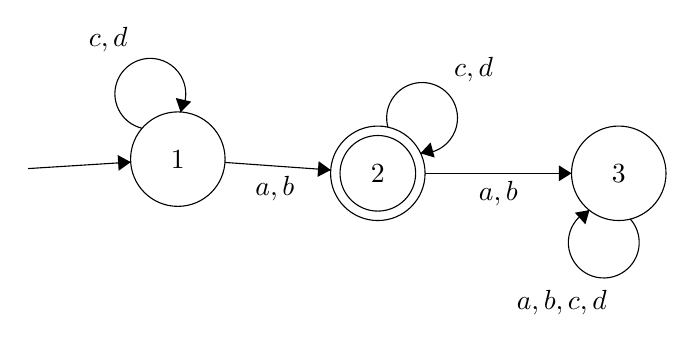
\begin{tikzpicture}[scale=0.2]
\tikzstyle{every node}+=[inner sep=0pt]
\draw [black] (14.7,-11.8) circle (3);
\draw (14.7,-11.8) node {$1$};
\draw [black] (27.4,-12.7) circle (3);
\draw (27.4,-12.7) node {$2$};
\draw [black] (27.4,-12.7) circle (2.4);
\draw [black] (42.7,-12.7) circle (3);
\draw (42.7,-12.7) node {$3$};
\draw [black] (5.2,-12.4) -- (11.71,-11.99);
\fill [black] (11.71,-11.99) -- (10.88,-11.54) -- (10.94,-12.54);
\draw [black] (12.441,-9.843) arc (256.83365:-31.16635:2.25);
\draw (10.28,-5.05) node [above] {$c,d$};
\fill [black] (14.88,-8.82) -- (15.55,-8.15) -- (14.57,-7.92);
\draw [black] (17.69,-12.01) -- (24.41,-12.49);
\fill [black] (24.41,-12.49) -- (23.64,-11.93) -- (23.57,-12.93);
\draw (20.86,-12.87) node [below] {$a,b$};
\draw [black] (28.041,-9.781) arc (195.34019:-92.65981:2.25);
\draw (33.48,-6.93) node [above] {$c,d$};
\fill [black] (30.11,-11.43) -- (31.01,-11.7) -- (30.75,-10.74);
\draw [black] (30.4,-12.7) -- (39.7,-12.7);
\fill [black] (39.7,-12.7) -- (38.9,-12.2) -- (38.9,-13.2);
\draw (35.05,-13.2) node [below] {$a,b$};
\draw [black] (43.425,-15.599) arc (41.76925:-246.23075:2.25);
\draw (39.08,-20.09) node [below] {$a,b,c,d$};
\fill [black] (40.84,-15.04) -- (39.91,-15.2) -- (40.58,-15.94);
\end{tikzpicture}
\end{center}

\subsection{}
$(c|d)^*|((c|d)^*(a|b)(c|d)^*)$

\subsection{}
This is ad-hoc but oh well.

\begin{lstlisting}
S -> CD AB CD
CD -> c CD | d CD | <empty>
AB -> a | b | <empty>
\end{lstlisting}

\section{Exercise}
\subsection{}
\begin{lstlisting}
S -> a S e
   | b S e
   | c S
   | d S
   | <empty>
\end{lstlisting}

\subsection{}
\begin{center}
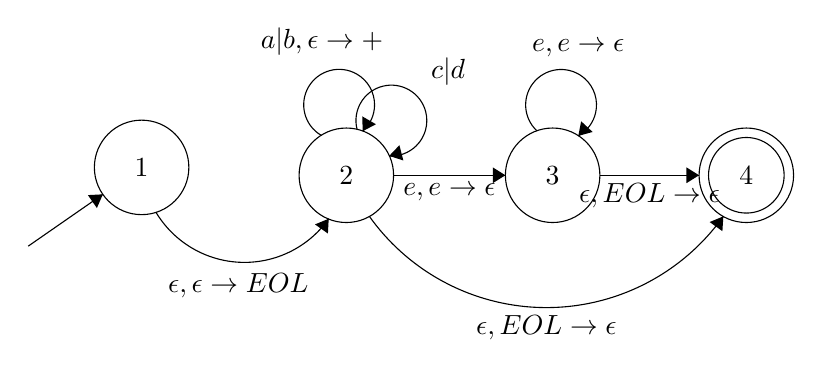
\begin{tikzpicture}[scale=0.2]
\tikzstyle{every node}+=[inner sep=0pt]
\draw [black] (14.7,-17.9) circle (3);
\draw (14.7,-17.9) node {$1$};
\draw [black] (27.7,-18.4) circle (3);
\draw (27.7,-18.4) node {$2$};
\draw [black] (40.8,-18.4) circle (3);
\draw (40.8,-18.4) node {$3$};
\draw [black] (53.1,-18.4) circle (3);
\draw (53.1,-18.4) node {$4$};
\draw [black] (53.1,-18.4) circle (2.4);
\draw [black] (7.5,-22.9) -- (12.24,-19.61);
\fill [black] (12.24,-19.61) -- (11.29,-19.66) -- (11.86,-20.48);
\draw [black] (26.583,-21.156) arc (-35.17937:-149.22582:6.55);
\fill [black] (26.58,-21.16) -- (25.71,-21.52) -- (26.53,-22.1);
\draw (20.84,-24.6) node [below] {$\epsilon,\epsilon\rightarrow EOL$};
\draw [black] (51.637,-21.012) arc (-35.47381:-144.52619:13.798);
\fill [black] (51.64,-21.01) -- (50.77,-21.37) -- (51.58,-21.95);
\draw (40.4,-27.3) node [below] {$\epsilon,EOL\rightarrow\epsilon$};
\draw [black] (26.112,-15.869) arc (239.83824:-48.16176:2.25);
\draw (26.15,-10.82) node [above] {$a|b,\epsilon\rightarrow+$};
\fill [black] (28.74,-15.6) -- (29.58,-15.16) -- (28.71,-14.66);
\draw [black] (28.383,-15.491) arc (194.52754:-93.47246:2.25);
\draw (34.16,-12.7) node [above] {$c|d$};
\fill [black] (30.42,-17.17) -- (31.32,-17.46) -- (31.07,-16.49);
\draw [black] (30.7,-18.4) -- (37.8,-18.4);
\fill [black] (37.8,-18.4) -- (37,-17.9) -- (37,-18.9);
\draw (34.25,-18.9) node [below] {$e,e\rightarrow\epsilon$};
\draw [black] (39.806,-15.582) arc (227.15723:-60.84277:2.25);
\draw (42.43,-10.92) node [above] {$e,e\rightarrow\epsilon$};
\fill [black] (42.43,-15.9) -- (43.34,-15.65) -- (42.61,-14.97);
\draw [black] (43.8,-18.4) -- (50.1,-18.4);
\fill [black] (50.1,-18.4) -- (49.3,-17.9) -- (49.3,-18.9);
\draw (46.95,-18.9) node [below] {$\epsilon,EOL\rightarrow\epsilon$};
\end{tikzpicture}
\end{center}

$1,2,2,2,3,3,4$

\section{Exercise}
We choose the word $a^pe^p \in L'$ which is clearly of longer than p. Since $|xy| \leq p$, $z = e^p$ and $y = a^q$, where $1 \leq q \leq p$, as $|y| > 0$. This means that $xy^0z = a^{p-q}e^p \notin L'$.

\section{Exercise}
\subsection{}
\begin{align*}
        s(s(s(0))) + s(s(0)) & \Rightarrow s(s(0)) + s(s(s(0))) & [r_3] \\
                             & \Rightarrow s(0) + s(s(s(s(0)))) & [r_1] \\
                             & \Rightarrow 0 + s(s(s(s(s(0))))) & [r_1] \\
                             & \Rightarrow s(s(s(s(s(0)))))     & [r_2] \\
\end{align*}

\subsection{}
\begin{equation}
        [r_5] \quad a_1 * a_2 \Rightarrow a_2 * a_1
\end{equation}
\begin{equation}
        [r_6] \quad 0 * a_1 \Rightarrow 0
\end{equation}
\begin{equation}
        [r_7] \quad s(0) * a_1 \Rightarrow a_1
\end{equation}
\begin{equation}
        [r_8] \quad s(n_1) * a_1 \Rightarrow n_1 * a_1 + a_1
\end{equation}

\subsection{}
\begin{align*}
        s(s(0)) * s(s(0)) & \Rightarrow s(0) * s(s(0)) + s(s(0)) & [r_8] \\
                          & \Rightarrow s(s(0)) + s(s(0))        & [r_7] \\
                          & \Rightarrow s(0) + s(s(s(0)))        & [r_1] \\
                          & \Rightarrow 0 + s(s(s(s(0))))        & [r_1] \\
                          & \Rightarrow s(s(s(s(0))))            & [r_2] \\
\end{align*}

\section{Exercise}
\subsection{}
When declaring a procedure using fully static scope rules we save both the current variables environment and procedure environment. And these are retrieved when calling a procedure. Thus we can make the following bindings as seen in Figure \ref{fig:fullystatic}, and figure out that $y = 3$.

\begin{figure}
        \centering
        \includegraphics[width=0.5\textwidth]{fullystatic.png}
        \caption{fully static scope bindings.}
        \label{fig:fullystatic}
\end{figure}

\subsection{}
In a fully dynamic scope we only save the procedure when we declare, and in the call of the procedure we simply use the variables and procedures in their respective current environments. Again we can draw the bindings as can be seen on Figure \ref{fig:fullydynamic}. Thus in this case $y=4$

\begin{figure}
        \centering
        \includegraphics[width=0.5\textwidth]{fullydynamic.png}
        \caption{fully dynamic scoping.}
        \label{fig:fullydynamic}
\end{figure}

\subsection{}
With these scope rules we will save the procedure environment when declaring a procedure, but use the current variable environment when calling one. On Figure \ref{fig:mixed} i have again shown the bindings. This time $y=5$

\begin{figure}
        \centering
        \includegraphics[width=0.5\textwidth]{mixed.png}
        \caption{Mixed scoping rules.}
        \label{fig:mixed}
\end{figure}

\section{Introduction}
This is time for all good men to come to the aid of their party!

\begin{prooftree}
        \infer0[by num]{\num{\underline{2}} \rightarrow 2}
        \infer0[by num]{\num{\underline{2}} \rightarrow 2}
        \infer2[by Plus]{\underline{2} + \underline{2} \rightarrow 4}
\end{prooftree}

\end{document}
